\documentclass[a4paper,10pt]{article}
\usepackage[utf8]{inputenc}

% ----  Useful packages % ---- 
\usepackage{amsmath}
\usepackage{graphicx}
\graphicspath{{images/}}
\usepackage{amsfonts}
\usepackage{amsthm}
\usepackage{amssymb}
\usepackage{makecell}
% ----  Useful packages % ---- 

\usepackage{wrapfig}
\usepackage{caption}
\usepackage{subcaption}
\usepackage{hyperref}
\hypersetup{
	colorlinks,
	citecolor=black,
	filecolor=black,
	linkcolor=black,
	urlcolor=black
}

% ---- Set page size and margins replace ------
\usepackage[letterpaper,top=2cm,bottom=2cm,left=3cm,right=3cm,marginparwidth=1.75cm]{geometry}
% ---- Set page size and margins replace ------

% ------- NOTA ------
\theoremstyle{remark}
\newtheorem{note}{Note}[subsection]
% ------- NOTA ------

% ------- OSSERVAZIONE ------
\theoremstyle{definition}
\newtheorem{observation}{Osservazione}[subsection]
% ------- OSSERVAZIONE ------

% ------- DEFINIZIONE ------
\theoremstyle{plain}
\newtheorem{definition}{Definizione}[subsection]
% ------- DEFINIZIONE ------

% ------- ESEMPIO ------
\theoremstyle{definition}
\newtheorem{example}{Esempio}[subsection]
% ------- ESEMPIO ------

% ------- DIMOSTRAZIONE ------
\theoremstyle{definition}
\newtheorem{demostration}{Dimotrazione}[subsection]
% ------- DIMOSTRAZIONE ------

% ------- TEOREMA ------
\theoremstyle{definition}
\newtheorem{theorem}{Teorema}[subsection]
% ------- TEOREMA ------

% ------- COROLLARIO ------
\theoremstyle{plain}
\newtheorem{corollaries}{Corollario}[theorem]
% ------- COROLLARIO ------

% ------- PROPOSIZIONE ------
\theoremstyle{plain}
\newtheorem{proposition}{Proposizione}[subsection]
% ------- PROPOSIZIONE ------

% ---- Footer and header ---- 
\usepackage{fancyhdr}
\pagestyle{fancy}
\fancyhf{}
\fancyhead[LE,RO]{A.A 2023-2024}
\fancyhead[RE,LO]{Green Computing}
\fancyfoot[RE,LO]{\rightmark}
\fancyfoot[LE,RO]{\thepage}

\renewcommand{\headrulewidth}{.5pt}
\renewcommand{\footrulewidth}{.5pt}
% ---- Footer and header ---- 

% ----  Language setting ---- 
\usepackage[italian, english]{babel}
% ----  Language setting ---- 

\usepackage{listings}
\usepackage{color}

\definecolor{dkgreen}{rgb}{0,0.6,0}
\definecolor{gray}{rgb}{0.5,0.5,0.5}
\definecolor{mauve}{rgb}{0.58,0,0.82}

\lstset{frame=tb,
	language=C,
	aboveskip=3mm,
	belowskip=3mm,
	showstringspaces=false,
	columns=flexible,
	basicstyle={\small\ttfamily},
	numbers=none,
	numberstyle=\tiny\color{gray},
	keywordstyle=\color{blue},
	commentstyle=\color{dkgreen},
	stringstyle=\color{mauve},
	breaklines=true,
	breakatwhitespace=true,
	tabsize=3
}

\title{\textbf{Green Computing}}
\author{Realizzato da: Ghirardini Filippo}
\date{A.A. 2023-2024}

\begin{document}
	\begin{titlepage} %crea l'enviroment
	\begin{figure}[t] %inserisce le figure
		\centering
\includegraphics[width=0.98\textwidth]{marchio_unipi_pant541.png}
	\end{figure}
	\vspace{20mm}
	
	\begin{Large}
		\begin{center}
			\textbf{Dipartimento di Informatica\\ Corso di Laurea Triennale in Informatica\\}
			\vspace{20mm}
			{\LARGE{Corso a Libera Scelta - 6 CFU}}\\
			\vspace{10mm}
			{\huge{\bf Computer Graphics}}\\
		\end{center}
	\end{Large}
	
	
	\vspace{36mm}
	%minipage divide la pagina in due sezioni settabili
	\begin{minipage}[t]{0.47\textwidth}
		{\large{\bf Professore:}\\ \large{Prof. }}
	\end{minipage}
	\hfill
	\begin{minipage}[t]{0.47\textwidth}\raggedleft
		{\large{\bf Autore:}\\ \large{Filippo Ghirardini}}
	\end{minipage}
	
	\vspace{25mm}
	
	\hrulefill
	
	\vspace{5mm}
	
	\centering{\large{\bf Anno Accademico 2023/2024 }}
	
\end{titlepage}
	
	\tableofcontents
	\newpage
	\maketitle
	\begin{center}
		\vspace{-20pt}
		\rule{11cm}{.1pt} 
	\end{center}
	\section{Punto materiale}
Oggetto caratterizzato da una massa [kg] e da un vettore posizione [m] nello spazio 3D.
Dimensioni trascurabili, forma irrilevante rispetto ai fenomeni di interesse.
Vettore posizione come funzione del tempo t[s].
\begin{example}
    Una molecola di ossigeno se sono interessato all'aereodinamica di una vettua. 
    Un satellite attorno alla terra se ignoro le forze di marea.
\end{example}
\hspace{-15pt}\textbf{Un vettore posizione} è una funzione del tempo $t[s]$.
$$\vec{r(t)} = (x(t), y(t), z(t)) = x(t)\hat{x} + y(t)\hat{z} + z(t)\hat{z}$$
\begin{observation}
    I versori cartesiani sono costanti
\end{observation}

\begin{definition}[Legge oraria]
    Si definisce come legge oraria la funzione $t \mapsto \vec{r}(t)$.
\end{definition}

\begin{definition}[Traiettoria]
    Il luogo geometrico di punti visitati dal punto materiale.
    $$\{\vec{r}(t)\:\: per \: t \in \mathbb{R}\}$$
\end{definition}

\begin{example}
    $\vec{r}(t) = (v_0t, y_0, 0)$ e $v_0 = 3m/s, y_o = 5m$ 
    \begin{figure}[h!]
        \centering
        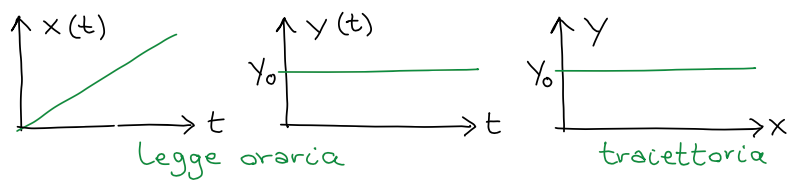
\includegraphics[width=0.8\textwidth]{images/ess-traiettoria.png}
    \end{figure}
\end{example}

\begin{definition}
    La \textbf{velocità istantanea} è la derivata della posizione rispetto al tempo.
    $$v = \lim_{\Delta t \to 0}\frac{\Delta s}{\Delta t} = \frac{ds}{dt}$$
\end{definition}

\begin{definition}
    La \textbf{velocità media} è definita come il rapporto tra lo spostamento e l'intervallo di tempo necessario per effettuarlo.
    $$v_m = \frac{\Delta s}{\Delta t}$$
\end{definition}
\hspace{-15pt}In parole povere è una grandezza che ci dice con quale rapidità cambia la posizione di un punto rispetto al tempo nell'instante $t$.
\subsection*{Vettore velocità}
Derivata rispetto al tempo del vettore posizione e si indica come 
$\frac{d\vec{r}(t)}{dt}\text{ oppure }\dot{\vec{r}}(t)[m/s]$
\begin{equation}
    \begin{split}
    \dot{\vec{r}}(t) & = (\dot{x}(t), \dot{y}(t), \dot{z}(t)) \\
     & = \frac{d}{dt}[x(t)\hat{x} + y(t)\hat{y} + z(t)\hat{z}] \\
     & = \dot{x}(t)\hat{x} + \dot{y}(t)\hat{y} + \dot{z}(t)\hat{z}
    \end{split}
\end{equation}
Per ricavare la forma esplicita uso le proprietà delle derivate (\textbf{linearità}, \textbf{Leibnitz})
\begin{example}
    $\vec{r}(t) = (v_0t, y_0, 0) = v_0t\hat{x} + y_0\hat{y}$ \:\:\:abbiamo che \:\:\:
    $\dot{\vec{r}}(t) = (v_0, 0, 0) = v_0 \hat{x}$
\end{example}
\hspace{-15pt}Velocità e spazio percorso ("integrale di linea").\\
\begin{wrapfigure}[3]{l}{5cm}
    \centering
    \includegraphics[width=5cm]{images/vettore-velocità.png}
\end{wrapfigure}
\begin{align*}
    L & = ||\vec{r}(t_1) - \vec{r}(t_0)|| + ||\vec{r}(t_2) - \vec{r}(t_1)|| + ||\vec{r}(t_3) - \vec{r}(t_2)|| + \dots \\
    & = \sum_i ||\vec{r}(t_{i+1} - \vec{r}(t_i)|| \:\: per\:\: |t_{i+1} - t_i| \text{"piccolo"} \\
    & = \sum_i ||\frac{\vec{r}(t_{i+1}) - \vec{r}(t_i)}{t_{i+1} - t_i}|| (t_{i+1} - t_i) = \int_{t_{in}}^{t_{f_{in}}}||\dot{\vec{r}}(t)||\\
\end{align*}
\begin{example}
    $\vec{r}(t) = (v_0t, y_0)\:\:\: \dot{\vec{r}}(t) = (v_0, 0)$\hspace{15pt}
    $||\dot{\vec{r}}(t)|| = \sqrt{v_0^2 + 0^2} = |v_0|$ \:\:\: $L = |v_0| \cdot (t_{f_{in}} - t_{in})$\\
    Il vettore è costante quindi facendo la derivata torna zero. Con la velocità si calcolo lo spazio percorso ("integrale di linea").
    La differenza fra le posizioni e la differenza dei tempi è il rapporto incrementale in caso gli intervalli siano sufficentemente
    piccoli, da qui si ottiene l'integrale.
\end{example}

\subsection{Vettore accelerazione}
Derivata rispetto al tempo del vettore velocità e si indica con $\frac{d^2\vec{r}(t)}{dt} \text{ oppure } \ddot{\vec{r}}(t) [m/s^2]$
\begin{equation}
    \ddot{\vec{r}}(t) = (\ddot{x}(t), \ddot{y}(t), \ddot{z}(t))\:\: = \:\: \ddot{x}(t)\hat{x} + \ddot{y}(t)\hat{y} + \ddot{z}(t)\hat{z}
\end{equation}
\begin{example}
    $\vec{r}(t)= (\frac{1}{2}a_0t^2, v_0t, 0)$ \hspace{10pt} $\dot{\vec{r}}(t) = (a_0t, v_0, 0)$ \hspace{10pt} $\dot{\vec{r}}(t) = (a_0, 0, 0)$
\end{example}
\hspace{-15pt}Serve perché l'equazione "del moto" di Newton che determinata la legge oraria è formulata in termini di accelerazione.

\subsection{Vettore quantità di moto}
Il prodotto di massa [kg] e velocità [m/s]
$$\vec{p}(t) = m \cdot \dot{\vec{r}}(t) = (m\dot{x}(t), m\dot{y}(t), m\dot{x}(t)) = m\dot{\vec{x}}(t)x + m\dot{\vec{y}}(t)y + m \dot{\vec{z}}(t)z$$
\begin{example}
    Prendiamo un punto di massa 2kg e velocità 3m/s lungo $\hat{x}$.\\
    $p_x(t) = 2 \cdot 3 kg\cdot m/s = 6 kg \cdot m/s$ \hspace{15pt} $p_y(t) = p_z(t) = 0$.
\end{example}
\hspace{-15pt}Serve per generalizzare l'equazione di Newton e per trattare sistemi di piu punti materiali.

\subsection{Vettore momento angolare rispetto a un polo P}
$$\vec{L}_p(t) = m(\vec{r}(t) - \vec{r}_p) \times \dot{\vec{r}}(t)$$
Dove $\vec{r}_p$ è il vettore posizione di p, mentre $\dot{\vec{r}}(t)$ è il prodotto vettoriale.
\begin{example}
    $\vec{r}_p = (l_0, 0, 0)$ \hspace{15pt} $\vec{r}(t) = (v_0t, y_0, 0)$\\
    $\vec{L}_p = m[(v_0t - l_0)\hat{x} + y_0\hat{y}] \times (v_0\hat{x}) \:\: = \:\: m(v_0t - l_0)v_0 \hat{x} \times \hat{x} + my_0v_0\hat{y}\times \hat{x} 
    \:\: = \:\: my_0v_0(-\hat{z}) = (0,0, -my_0v_0)$\\
    Ricorda che $\hat{x} \times \hat{x} = 0$ e $\hat{y} \times \hat{x} = -\hat{z}$
\end{example}
\hspace{-15pt}Il momento angolare dice quanta inerzia ha un oggetto in una rotazione (descrizione sommaria).\\
Il polo P è parte della definizione. È una scelta! Il risultato dipende dal polo.
Serve per formulare l'equazione del moto di sistemi di punti materiali e corpi rigidi.

\subsection{Coordinate polari}
Un metodo per rapprensentare delle cordinate x, y andando a misurare prima la distanza dall'origine e poi si va a vedere
quanto vale l'angolo fra questo segmento dall'asse x, utilizzando seno e coseno.
\begin{wrapfigure}[7]{l}{2cm}
    \centering
    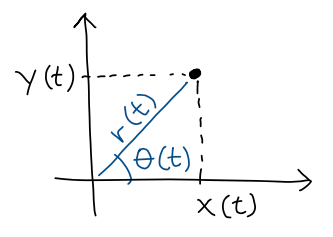
\includegraphics[width=5.5cm]{images/coordinate-polari.png}
\end{wrapfigure}
\begin{align*}
    \begin{cases}
        x(t) = r(t) \cdot \cos(\Theta(t))\\
        y(t) = r(t) \cdot \sin(\Theta(t)) 
    \end{cases}
\end{align*}
\begin{align*}
    \begin{cases}
        r(t) = \sqrt{x(t)^2 + y(t)^2} \geq 0\\
        tg(\Theta(t)) = y(t) / x(t) 
    \end{cases}
\end{align*}
\\
\begin{example} Esempi di rappresentazione di coordinate in coordinate polari.\\
    $x = 0, y = l_0 > 0 \:\: \Rightarrow \:\: r = l_0, \Theta = \pi/2$\\
    $x = 0, y = -l_0 < 0 \:\: \Rightarrow \:\: r = l_0, \Theta = -\pi/2$\\
    $x = l_0, y = l_0 > 0 \:\: \Rightarrow \:\: r = \sqrt{2}l_0, \Theta = \pi/4$\\
\end{example}

\subsection{Versori polari (2D)}
Definisco un versore $\hat{r}(t)$ che punta verso il punto materiale e un versore $\hat{\Theta}(t)$ ortogonale.
Si esprime facilmente in coordinte polari.
$$\vec{r}(t) = (x(t), y(t)) = (r(t)\cos \Theta(t), r(t)\sin\Theta(t)) \:\: = \:\: r(t)(\cos\Theta(t)\hat{x} + \sin\Theta(t)\hat{y})$$
Ma $||\vec{r}(t)|| = |r(t)| = r(t)$ allora definisco $\hat{r}(t) = \vec{r}(t)/ ||\vec{r}(t)|| = \cos \Theta(t)\hat{x} + \sin\Theta(t)\hat{y}$\\\\
Trovo facilmente che un versore ortogonale è:
$$\hat{\Theta(t)} = -\sin\Theta(t)\hat{x} + \cos\Theta(t)\hat{y} \:\:\:\text{infatti} \:\:\: \hat{r}\cdot \hat{\Theta} = c \cdot (-s) + s \cdot c = 0$$
\begin{wrapfigure}[7]{r}{6cm}
    \centering
    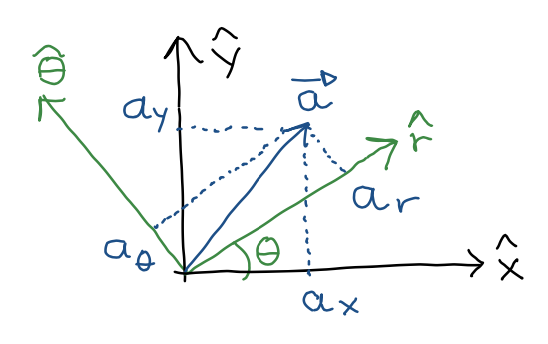
\includegraphics[width=5.5cm]{images/trasformazioni-inverse.png}
\end{wrapfigure}
\begin{note}
    Non c'è legame fra $\Theta$ e $\hat{\Theta}$ è solo una convenzione.
\end{note}
\hspace{-15pt}Le trasformazioni inverse invece si fanno come segue (verifico per sostituzione):
$$\hat{y} = \cos\Theta(t)\hat{r} - \sin\Theta(t)\hat{\Theta} \hspace{20pt} \hat{y} = \sin\Theta(t)\hat{r} + \cos\Theta(t)\hat{\Theta}$$
Possono quindi scrivere ogni vettore nella forma $\vec{a} = a_r\hat{r} + a_{\Theta}\hat{\Theta}$ con le componenti polari $a_r, a_{\Theta}$.
Per evitare ambiguità non scriviamo $(a_r, a_{\Theta})$ e riserviamo la notazione alle componenti cartesiane.\\\\
A differenza dei versori cartesiani quelli polari dipendono dal tempo per costruzioni.
$$\dot{\hat{r}}(t) = \frac{d}{dt}[\cos\Theta(t) \hat{x} + \sin\Theta(t)\hat{y}] \:\: = \:\: -\sin\Theta(t) \cdot \dot{\Theta}(t)\hat{x} + \cos\Theta(t) \cdot \dot{\Theta}(t)\hat{y}$$
Dove $\cos\Theta(t) \cdot \dot{\Theta}(t)$ si applica la derivata della somma, Leibnitz, funzione composta.
$$= \dot{\Theta}(t)\cdot \hat{\Theta}(t) \:\:\:\:(\text{confronto l'espressione di} \hat{\Theta}(t))$$
Similmente $\dot{\hat{\Theta}}(t)= - \dot{\Theta}\hat{r}(t)$.


\subsection*{Vettori posizione, velocità, accelerazione}
$$\vec{r}(t) = r(t)\hat{r}(t)$$
Dove abbiamo che $\vec{r}(t)$ è il vettore, $r(t)$ è una coordinata polare, $\hat{t}(t)$ è il versore polare.
$$\dot{\vec{r}}(r) = \dot{r}(t)\hat{r}(t) + r(t)\dot{\Theta}(t)\hat{\Theta}(t)$$
Dove la parte $\dot{\vec{r}}(r)$ è la velocità radiale.
$$\ddot{\vec{r}}(t) = [\ddot{r}(t) - r(t)\dot{\Theta}(t)^2] \hat{r} + [r(t) \ddot{\Theta}(t) + 2\dot{r}(t)\dot{\Theta}(t)]\hat{\Theta}$$
Nel quale abbiamo che la parte $r(t)\dot{\Theta}(t)^2$ si chiama \textbf{velocità centripeta}, mentre $2\dot{r}(t)\dot{\Theta}(t)$ si dice \textbf{accelerazione di Coriolis}.


	% !TeX spellcheck = it_IT
\newpage
\section{Green Computing}
In generale, il green computing può aiutare le organizzazioni a ridurre l'impatto ambientale e a risparmiare sui costi energetici e di gestione.

\begin{definition}[Green Computing]
	Il green computing tratta la \textbf{progettazione}, la \textbf{realizzazione} e l'\textbf{utilizzo} di \underline{sistemi ICT}, \underline{computer} e \underline{dispositivi elettronici}\footnote{Tutti quei dispositivi che si appoggiano all'informatica per funzionare, e.g. aspirapolvere} in modo responsabile e sostenibile dal punto di vista ambientale, considerando in particolare il \textbf{consumo energetico} e \textbf{impronta di carbonio}.
\end{definition}

\begin{definition}[$CO_2$-eq]
	L'anidride carbonica equivalente è una misura che esprime l'impatto di una certa quantità di gas serra rispetto alla stessa quantità di anidride carbonica.
\end{definition}

\begin{definition}{Energy Star}
	Il progetto Energy Star nasce negli anni '90 ed è stata una delle prime iniziative relative al green computing per dare un indicatore dell'efficienza energetica. Il problema principale è che è \textbf{facoltativo}.
\end{definition}

\subsection{Approccio olistico}
Per funzionare segue un approccio \textbf{olistico}, analizzando tutto il \textbf{ciclo di vita} di un sistema, sia \emph{vericalmente} che \emph{orizzontalmente}.

\begin{itemize}
	\item \textbf{Progetto}: progettare in modo sostenibile computer, server, sistemi di raffreddamento e software a basso consumo e alta efficienza.
	\item \textbf{Produzione}: attenzione a non sprecare risorse limitate, ridurre gli scarti di fabbricazione e utilizzare fonti rinnovabili per la produzione.
	\item \textbf{Trasporto}: cercare di ridurre e ammortizzare l'uso di carburanti fossili sostituendoli con veicoli elettrici o ibridi e facendo spedizioni accorpate.
	\item \textbf{Uso}: utilizzare i sistemi cercando di ridurre il consumo con politiche di risparmio (e.g. ibernazione)
	\item \textbf{Dismissione}: lo smaltimento di dispositivi elettronici attraverso il riciclo
\end{itemize}

\subsection{Pilastri fondamentali}
\begin{center}
	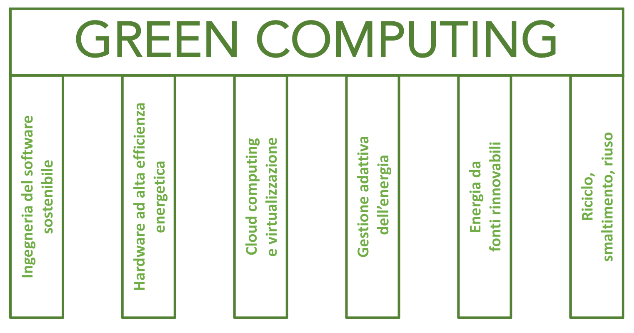
\includegraphics[scale=0.5]{green_pilastri.png}
\end{center}
\subsubsection{Ingegneria del software sostenibile}
È possibile fare in modo che i programmi consumino meno energia e che il loro dispiegamento nelle varie fasi del ciclo di vita produca minori gas inquinanti. In particolare, programmare \emph{sfruttando le peculiarità di linguaggi e hardware} che possano rendere il software più disponibile.
\subsubsection{Hardware ad alta efficienza energetica}
L'hardware ad alta \textbf{efficienza energetica} o le configurazioni Eco permettono di ridurre l'impatto ambientale e risparmiare sui costi energetici e di gestione. Inoltre, sistemi di raffreddamento più efficienti e processori di nuova generazione consumano meno. Alcune \textbf{periferiche} a basso consumo energetico sono:
\begin{itemize}
	\item Schermi OLED:  I pixel dello schermo si spengono su immagini nere risparmiando energia
	\item Stampanti, scanner, etc.
\end{itemize}
Va considerato un trade-off tra prestazioni e consumi, con l'obiettivo di avere un minore impatto ambientale
\subsubsection{Cloud computing e virtualizzazione}
Il Cloud Computing permette di \textbf{condividere} le risorse informatiche tra più utenti e organizzazioni, riducendo così gli sprechi di risorse. Inoltre, le grandi aziende che forniscono servizi cloud possono permettersi di investire in infrastrutture tecnologiche più \textbf{efficienti} dal punto di vista energetico, per esempio utilizzando fonti rinnovabili per alimentare i propri data center. Inoltre, il cloud computing permette una maggiore \textbf{flessibilità} nell'allocazione delle risorse, garantendo l'accesso (anche elastico) solo alle risorse necessarie per un'applicazione specifica. Ciò si traduce in una riduzione del consumo energetico. La virtualizzazione delle risorse consente di \textbf{ottimizzare} l'utilizzo hardware, riducendo così gli sprechi.
\subsubsection{Gestione adattiva dell'energia}
La gestione adattiva dell'energia permette di abbattere i consumi e i costi tramite metodi su più livelli, appiattendo la curva di consumo energetico, risparmiando soldi e risorse e riducendol’utilizzo di energia nelle ore di basso utilizzo. Alcuni esempi sono:
\begin{itemize}
	\item \textbf{Adattività del raffreddamento}: ridurre/aumentare il raffreddamento in base all’utilizzo del processore, può portare fino ad una riduzione del 20\% dei consumi
	\item \textbf{Batteria}: aumento della vita della batteria evitando di stressarla utilizzando l’energia della presa quando in carica
	\item \textbf{Sistemi operativi}: Adaptive job scheduling e timing di spegnimento e sospensione dello schermo e del sistema
	\item \textbf{Illuminazione adattiva dei dispositivi mobil}i: la maggior parte dei nuovi dispositivi sono in grado di adattare la luminosità del display in base alla luminosità ambientale
\end{itemize}
\subsubsection{Energia da fonti rinnovabili}
La transizione verde ha come pilastro fondamentale il passaggio da un sistema basato per la quasi totalità su fonti energetiche inquinanti a un modello virtuoso incentrato invece su fonti rinnovabili. Utilizzare \textbf{fonti rinnovabili} per alimentare i data center e i dispositivi informatici può quindi ridurre significativamente le emissioni di CO2 e 
contribuire a combattere il cambiamento climatico.
\subsubsection{Riciclo, smaltimento, riuso}
È possibile \textbf{sensibilizzare} l'utente sul giusto uso dei mezzi a sua disposizione e quindi della loro conseguente fine di utilizzo. Ottimizzare l'impiego dei dispositivi porta una determinante longevità, minimizzando quindi il rifiuto.
\begin{itemize}
	\item Inoltre, per ridurre la produzione di rifiuti è fondamentale \textbf{riutilizzare} (ad esempio rivendendo) i dispositivi elettronici ancora validi. In molti casi è sufficiente sostituire componenti degradati (e.g. le batterie) e mantenere il resto. Oltretutto molti dispositivi possono essere considerati obsoleti per certi scopi ma ancora ottimi per altri (e.g. server).
	\item È fondamentale ingegnerizzare il processo di \textbf{smaltimento} in modo da permettere il \textbf{riciclo} di parte dei componenti. Ad esempio dalle schede stampate si possono recuperare metalli preziosi come l'oro. La legislazione italiana necessita il corretto trattamento dei rifiuti per ridurre l'inquinamento. Di conseguenza anche la scelta di macchinari e strumenti mirati allo smaltimento è fondamentale per fare in modo che un'azienda possa essere ritenuta green.
	\item La tecnologia stessa può essere uno strumento potente per \textbf{sensibilizzare} il consumatore su queste tematiche e per fargli conoscere le aziende green.
\end{itemize}
\subsection{Applicazioni green}
Sfruttare i sistemi ICT per l'\textbf{ottimizzazione} di processi che sfruttano risorse limitate (e.g. combustibili fossili nel trasporto, energia elettrica nel riscaldamento, acqua potabile nell'irrigazione) è un aspetto importante del green computing.
	% !TeX spellcheck = it_IT
\newpage
\subsection{Ebook reader}
Entro il 2025 si prevede che gli e-reader rappresenteranno circa il $75\%$ del mercato totale, anche se allo stesso tempo il numero di libri cartacei prodotti e  venduti è in continuo aumento.

\subsubsection{Ciclo di produzione}
Vediamo il ciclo di vita di un libro tradizionale cartaceo
\begin{center}
	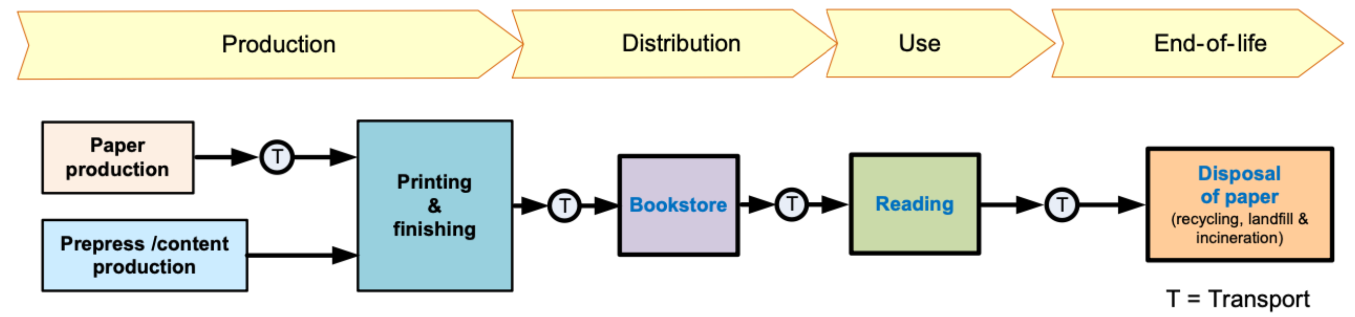
\includegraphics[scale=0.3]{books_lifecycle.png}
\end{center}
Le materie prime necessarie sono, per un libro a copertina morbida, $150-300$g di carta e $7.5$lt di acqua. Sono necessari $2$KWh  e la loro distribuzione (assumendo che non si usi la macchina per comprarlo) produce circa 10 volte quella della produzione. L'utilizzo è trascurabile dal punto di vista energetico in quanto al massimo serve una luce per leggere.
\begin{center}
	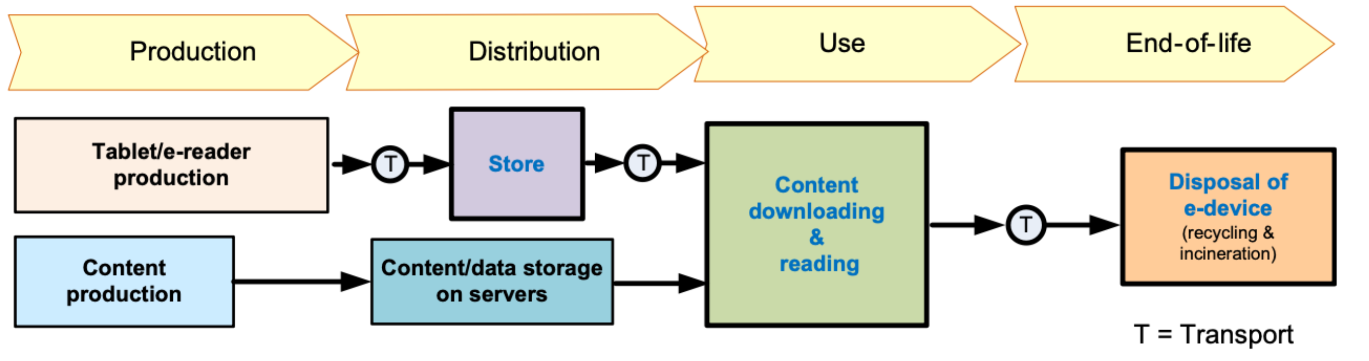
\includegraphics[scale=0.3]{ereader_lifecycle.png}
\end{center}
Per quanto riguarda invece gli e-book reader, sono necessari circa $15$Kg di materie prime (metalli rari, sabbia, etc...) e $300$lt di acqua (batterie, chip, oro dei circuiti). Sono necessari $100$KWh per la produzione e assumiamo i costi di distribuzione di un  \href{https://www.icao.int/environmental-protection/Carbonoffset/Pages/default.aspx}{\color{blue}volo Milano-Roma}.

\subsubsection{Confronto}
Considerando i dati precedenti:
\begin{enumerate}
	\item Quanti libri si producono con le materie prime necessarie per produrre un e-book reader?\\
	\begin{equation*}
		\frac{15Kg}{0.150Kg} = 100 \quad \frac{15Kg}{0.300Kg}=50
	\end{equation*}
	\item Quanti libri si producono con l'acqua necessaria per produrre un e-book reader?\\
	\begin{equation*}
		\frac{300lt}{7.5lt} = 40
	\end{equation*}
	\item Quanti libri si producono con l'energia necessaria per produrre un e-book reader?\\
	\begin{equation*}
		\frac{100KWh}{2KWh} = 50
	\end{equation*}
	\item Quanti libri serve produrre e trasportare per inquinare quanto per la produzione e il trasporto di un e-book reader?\\
	\begin{equation*}
		\begin{split}
			&\text{Produzione e-book reader}=0.319\frac{g}{Kw/h} \cdot 100Kw/h = 31.9Kg \quad \text{Distribuzione e-book reader}=41.8 Kg \\
			&\text{Totale e-book reader}=31.9Kg + 41.8Kg = 73.7 Kg \\
			&\text{Produzione libro}=0.319 \frac{g}{Kw/h} \cdot 2Kw/h = 0.638Kg \quad  \text{Distribuzione libro}= 0.638Kg \cdot 10 = 6.380Kg\\
			&\text{Totale libro}=6,380Kg + 0.638 Kg = 7.018Kg \\
			& \text{\textbf{Libri per e-book reader}}=\frac{73.7Kg}{7.018Kg}=10.5
		\end{split}
	\end{equation*}
	\item Qual'è la media dei valori delle risposte precedenti (quanti libri vale un e-book reader)?
	\begin{equation*}
		\frac{\frac{100+50}{2} + 40 + 50 + 10.5}{5} = 43.9
	\end{equation*}
	\item Quanti libri bisogna leggere all'anno per ammortizzare un e-book reader su 5 anni di vita media?
	\begin{equation*}
		\frac{43.9}{5} = 8.8
	\end{equation*}
\end{enumerate}

\subsubsection{Salute}
La produzione di libri ed e-book reader produce ossidi di azoto e zolfo %TODO FInisci

\subsubsection{Dismissione}
\begin{table}
	\begin{tabular}{|c|c|}
		\hline
		Libro & E-book reader \\
		\hline
		La \textbf{decomposizione} può generare il doppio delle emissioni e degli impatti tossici sulle falde acquifere rispetto alla sua intera produzione & In caso di smaltimento illegale in uno dei paesi in via di sviluppo, i lavoratori (spesso bambini) saranno esposti all'impatto tossico di alcune sostanza smantellate. \\
		Può essere prestato, regalato, donato ad una biblioteca oppure correttamente riciclato. & Se correttamente riciclato, molti materiali si potranno recuperare o smaltire correttamente.
	\end{tabular}
\end{table}
%TODO Formatta decentemente

\subsection{Blockchain}
Bitcoin nasce nel 2008 come prima tecnologia basata sulla blockchain.
\begin{definition}[Blockchain]
	Blockchain è un libro mastro distribuito in grado di registrare e validare transazioni in assenza di un’entità centrale (e.g. banca).
\end{definition}
In particolare una blockchain ha le seguenti caratteristiche:
\begin{itemize}
	\item \textbf{Distribuita}: tutti i nodi partecipanti ne conservano una copia per trasparenza
	\item \textbf{Immutabile}: i record nella catena non possono essere né modificati né cancellati
	\item \textbf{Marcata temporalmente}: ogni transazione ha un timestamp
	\item \textbf{Unanime}: tutti i nodi partecipanti devono riconoscere la validità delle transazioni
	\item \textbf{Anonima}: l’identità dei partecipanti non è rivelata
	\item \textbf{Sicura}: tutti i record vengono criptati individualmente
	\item \textbf{Programmabile} per mezzo di SmartContracts
\end{itemize}

\subsubsection{Proof of Work}
La blockchain si basa sul concetto per cui ogni blocco, composto dalla transazione e dal riferimento a quella precedente, possa essere aggiunto solo quando viene fornita una \textbf{proof of work} da parte dei minatori, che risolvono problemi difficili (e.g. scomposizione in fattori primi).\\
Quando viene richiesta una transazione si crea un blocco che viene distribuito a tutti i partecipanti.\\
La difficoltà della proof of work aumenta con l'aumentare delle capacità computazionali dei nodi che scrivono nella blockchain, in modo tale da equilibrare:
\begin{itemize}
	\item \textbf{Sicurezza}: ad esempio evitando attacchi di doppia-spesa, o aggiunta di blocchi falsi 
	\item \textbf{Velocità di esecuzione} delle transazioni (stabilita attorno ai 10 minuti)
\end{itemize}

\subsubsection{Hardaware}
La potenza hardware per Bitcoin si misura in \textbf{GigaHash} al secondo (un hash è un calcolo da risolvere). L'hardware necessario si è evoluto con il tempo:
\begin{itemize}
	\item 2008 - \textbf{CPU}, $0.01GH/s$ con un consumo di $2.5Wh/GH$
	\item 2009 - \textbf{GPU}, $0.2-2GH/s$
\end{itemize}

\subsubsection{Minatori}
Possiamo suddividere le categorie dei minatori in:
\begin{itemize}
	\item \textbf{Piccoli}, il $15\%$ del totale, con un consumo fino a $0.1MW$ per $0.9PH/s$
	\item \textbf{Medi}, il $19\%$ del totale, con un consumo tra $0.1MW$ e $1MW$ per $9PH/s$
	\item \textbf{Grandi}, il $66\%$ del totale, con un consumo maggiore di $1MW$ per oltre $9PH/s$
\end{itemize}

\subsubsection{Analisi}
Consideriamo che al 2019 il consumo dell'hardware più efficiente era di $1.4 \cdot 10^{-5} Wh/GH$ e che per raffreddarlo veniva utilizzato il $5\%$ del consumo. Il numero di hash eseguiti in un'ora a novembre del 2019 era di $3.56 \cdot 10^{11} TH$. La localizzazione geografica dei minatori era:
\begin{itemize}
	\item \textbf{Cina} con il $68\%$ ad un costo di $0.55 \frac{kgCO_2-eq}{kWH}$
	\item \textbf{EU} con l'$11\%$ ad un costo di $0.28 \frac{kgCO_2-eq}{kWH}$
	\item \textbf{Privati} con il $21\%$ ad un costo di $0.475 \frac{kgCO_2-eq}{kWH}$
\end{itemize}
Considerando queste informazioni
\begin{enumerate}
	\item Qual è un limite inferiore al consumo energetico annuo di Bitcoin?
	\begin{equation*}
		\begin{split}
			&\text{Consumo per hash}=1.4 \cdot 10^{-5} \frac{Wh}{GH} + 5\% = 1.47 \cdot 10^{-5} \frac{Wh}{GH} \\
			&\text{Consumo per ora}=1.47 \cdot 10^{-5} \frac{Wh}{GH}  \cdot 3.56 \cdot 10^{14} GH = 5.2332 \cdot 10^9 W = 5.2332 \cdot 10^6 kW \\
			&\textbf{Consumo annuo}=5.2332 \cdot 10^6 kWh * 8760h = 4.5842832 \cdot 10^{10} kWh
		\end{split}
	\end{equation*}
	\item Quante emissioni di carbonio vengono prodotte all'anno se si utilizza quel limite inferiore come stima?
	\begin{equation*}
		\begin{split}
			&\text{Consumo \textbf{Cina}}=4.5842832 \cdot 10^{10} kWh \cdot 0.68 \cdot 0.55 \frac{kgCO_2-eq}{kWH} = 1.7145219168 \cdot 10^{10} kgCO_2-eq\\
			&\text{Consumo \textbf{EU}}=4.5842832 \cdot 10^{10} kWh \cdot 0.11 \cdot 0.28 \frac{kgCO_2-eq}{kWH} = 1.4119592256 \cdot 10^{9} kgCO_2-eq\\
			&\text{Consumo \textbf{privati}}=4.5842832 \cdot 10^{10} kWh \cdot 0.21 \cdot 0.475 \frac{kgCO_2-eq}{kWH} = 4.572822492 \cdot 10^{9} kgCO_2-eq
		\end{split}
	\end{equation*}
\end{enumerate}

\subsubsection{Oggi}
Nella primavera del 2021 alcuni stati come la Cina proibiscono il mining di Bitcoin e questo ha aumentato l'intensità del mining del $43\%$ rispetto al 2019.
%TODO Inserisci grafici
%TODO Inserisci dati sulla carbon footprint	

Ad oggi esiste il \textbf{Crypto Climate Accord} che ha come obiettivo quello di contribuire a raggiungere gli Accordi di Parigi tramite l'utilizzo di energie rinnovabili entro il 2030.

\subsubsection{Conclusione}
La blockchain è una tecnologia all'avanguardia che potrebbe avere un impatto molto grande su molti settori. È importante eseguire un'analisi di costi e benefici per valutare se conviene o meno:
\begin{enumerate}
	\item \textbf{Emissioni} di carbonio
	\item Rischi di \textbf{centralizzazione}: se qualcuno ottenesse il $51\%$ della computing power avrebbe il controllo della blockchain
	\item Possibilità di \textbf{controllo} per evitare traffici illegali
\end{enumerate}

\subsubsection{Proof of Stake}
Per affrontare le problematiche indicate ai punti 1 e 2 si vorrebbe introdurre la \textbf{proof of stake}, dove l'abilità di minare è determinata in base alla quantità di moneta che un utente possiede. Il minatore non viene premiato con la moneta al completamento del calcolo ma con degli interessi. In questo modo si evita anche l'attacco del $51\%$ poiché si rende necessario avere il $51\%$ della moneta (più difficile).
	% !TeX spellcheck = it_IT
\newpage
\section{Performance}
Un modello per misurare le performance di un sistema ICT è il seguente:
\begin{center}
	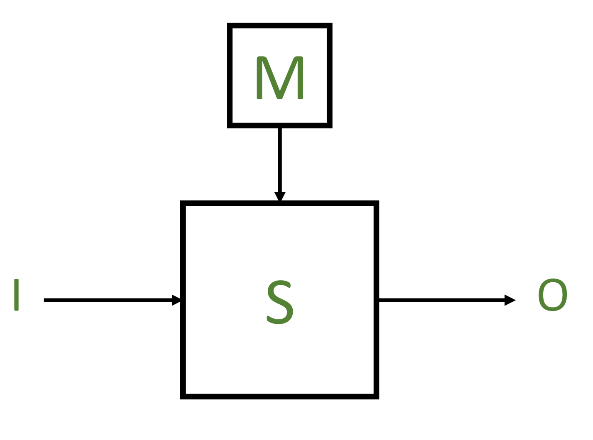
\includegraphics[scale=0.3]{performance_model.png}
\end{center}
in cui abbiamo degli \textbf{input} elaborati dal sistema che produce \textbf{output} è che viene monitorato per la \textbf{QoS} (Quality of Service) da un \textbf{monitor}.\\
Il \textbf{monitoraggio} di metriche di performance in un sistema ICT è fondamentale per garantirne il corretto funzionamento e necessita quindi di un \textbf{modello}. Queste metriche devono essere messe in corrispondenza con una \textbf{Quality of Service} da garantire, e viene fatto nel \textbf{Service Level Agreement} (SLA).

\subsection{Metriche}
\begin{definition}[Metrica]
	Si tratta della misurazione di una caratteristica (o di un insieme di esse) di un sistema che fornisce un'informazione utile.
\end{definition}
In sistemi complessi le metriche possono essere combinate mediante:
\begin{itemize}
	\item \textbf{Somma} (e.g. latenza)
	\item \textbf{Moltiplicazione} (e.g. disponibilità)
	\item \textbf{Max/Min} (e.g banda)
\end{itemize}

\subsubsection{Categorie}
Le metriche di performance di un sistema ICT si dividono in 4 categorie:
\begin{itemize}
	\item \textbf{Elaborazione} 
	\begin{itemize}
		\item \emph{Capacità di calcolo}: il massimo numero di richieste per unità di tempo che il sistema riesce a processare senza perdite
		\item \emph{Qualità}: la precisione ottenuta dai risultati
	\end{itemize}
	\item \textbf{Trasmissione} dati
	\begin{itemize}
		\item \emph{Banda}: il massimo throughput di dati supportato da un collegamento all'altro o lungo un cammino nella rete. La \emph{banda disponibile} si ottiene come differenza tra la \emph{banda nominale} e quella attualmente in uso
		\item \emph{Latenza}:  l’intervallo di tempo in cui si completa il trasferimento di dati
		lungo un collegamento o un cammino di rete
		\item \emph{Jitter}: la variazione di latenza tra richieste successive
		\item \emph{Packet loss}: la percentuale di pacchetti non ricevuti sul totale di
		pacchetti inviati
	\end{itemize}
	\item \textbf{Immagazzinamento} dati
	\begin{itemize}
		\item \emph{Capacità}: spazio a disposizione per salvare i dati
		\item \emph{Throughput}: massima quantità di dati che si riescono a
		scrivere/leggere per unità di tempo
	\end{itemize}
	\item \textbf{Qualità dell'esperienza} dell'utente. Spesso riportata su una scala da 1 a 5 e può includere \emph{disponibilità}, \emph{framerate}, \emph{qualità video}, etc.
\end{itemize}
\subsection{Efficienza energetica}
Dato il modello in precedenza, aggiungiamo l'\textbf{energia elettrica} utilizzata e l'\textbf{anidride carbonica} prodotta:
\begin{center}
	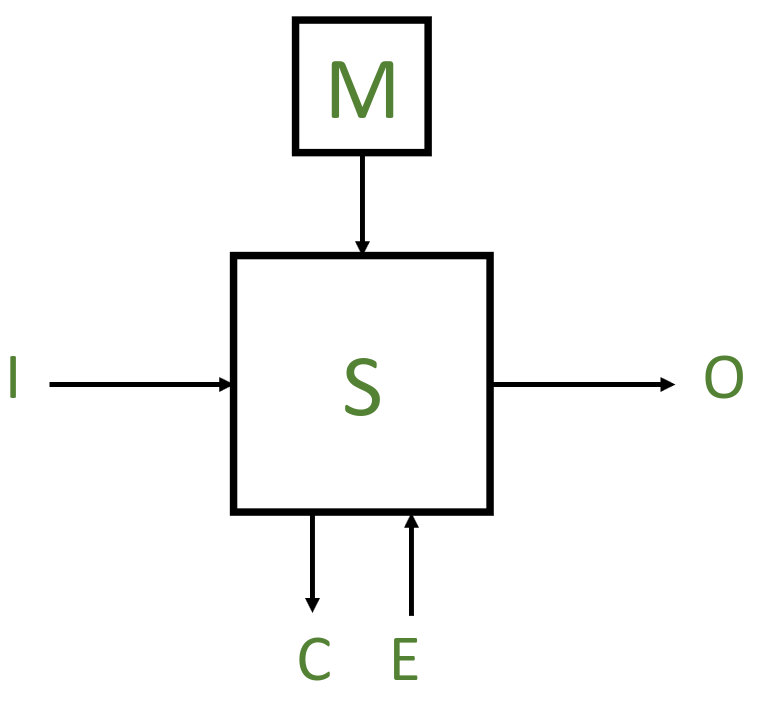
\includegraphics[scale=0.2]{performance_model_energy.png}
\end{center}
Un primo modo per valutare un sistema ICT dal punto di vista \emph{energetico} è tramite l'\textbf{efficienza}:
\begin{equation}
	\epsilon = \frac{\#calcoli}{E}=\bigg[\frac{FLOPS}{J}\bigg] \simeq \bigg[\frac{FLOPS}{W}\bigg]
\end{equation}

\begin{definition}[Legge di Koomey]
	La quantità di calcoli per Joule di energia raddoppia all'incirca ogni $1.5$ anni.
\end{definition}
La legge si è dimostrata vera fino al 2010 circa. Oggi raddoppia ogni $2.5$ anni si fermerà come quella di Moore e quella di Dennard.\\
Allo stesso modo la quantità di batteria necessaria per svolgere una certa quantità di calcoli diminuisce nel tempo (oggi di 16 volte ogni 10 anni).

\subsubsection{Power Usage Effectiveness}
L'energia consumata nel mondo ICT si divide in:
\begin{itemize}
	\item Per i \textbf{sistemi IT}
	\begin{itemize}
		\item Energia per alimentare server e dispositivi di rete
	\end{itemize}
	\item Per i \textbf{sistemi non IT}
	\begin{itemize}
		\item Sistemi di raffreddamento
		\item Sistemi di allarme e UPS
		\item Sistemi di illuminazione
	\end{itemize}
\end{itemize}
Per valutare l'efficienza di un sistema ICT si usa il Power Usage Effectiveness (PUE):
\begin{equation}
	PUE=\frac{P_{IT}+P_{non-IT}}{P_{IT}} = 1+\frac{P_{non-IT}}{P_{IT}}
\end{equation}

\subsubsection{Datacentre Infrastructure Efficiency}
L'inverso del PUE è detto Datacentre Infrastructure Efficiency (DCiE):
\begin{equation}
	DCiE=\frac{P_{IT}}{P_{IT}+P_{non-IT}}=\frac{1}{PUE}
\end{equation}

\newpage
Sia PUE che DCiE sono influenzati da:
\begin{itemize}
	\item \textbf{Utilizzo} del sistema nel \emph{tempo} e nello \emph{spazio}
	\item \textbf{Età} e \textbf{progettazione} del sistema
	\item \textbf{Efficienza} complessiva del sistema
\end{itemize}
Alcuni valori tipici sono:
\begin{table}[h]
	\centering
	\begin{tabular}{|c|c|c|}
		\hline
		\textbf{PUE} & \textbf{DCiE} & \textbf{Level of Efficiency} \\
		\hline
		$3.0$ & $33\%$ & Very inefficient \\
		\hline
		$2.5$ & $40\%$ & Inefficient \\
		\hline
		$2.0$ & $50\%$ & Average \\
		\hline
		$1.5$ & $67\%$ & Efficient \\
		\hline
		$1.2$ & $83\%$ & Very efficient \\
		\hline
	\end{tabular}
\end{table}
	% !TeX spellcheck = it_IT
\newpage
\section{Energia in un sistema ICT}
Prendiamo come riferimento il modello \textbf{olistico} di \emph{Drouant et al} proposto nel 2014.
\subsection{Energia}
L'energia si compone di:
\begin{equation}
	E = E_i + E_u + Ef
\end{equation}
dove:
\begin{itemize}
	\item \textbf{$E_i$} (iniziale) rappresenta l'energia necessaria per la \emph{progettazione} ($E_p$), \emph{produzione} ($E_m$) e \emph{trasporto al venditore} ($E_{ti}$)
	\item \textbf{$E_u$} (utilizzo) rappresenta l'energia necessaria per l'\emph{uso} e la \emph{gestione}
	\item \textbf{$E_f$} (finale) rappresenta l'energia necessaria al \emph{trasporto al centro di smaltimento} ($E_{tf}$) e il \emph{riciclo} ($E_r$)
\end{itemize}
Ottenendo quindi:
\begin{equation}
	E = (E_p + E_m + E_{ti}) + \int_{t=0}^{t=\text{fine vita}}P_u(t)dt + (E_{tf} + E_r)
\end{equation}
In particolare, l'integrale rappresenta la somma di quanto consuma in ogni istante di vita in un prodotto:
\begin{equation}
	\tilde{PUE} \cdot \int_{t=0}^{t=1_{year}} P_u(t)dt \simeq \tilde{PUE} \cdot \sum_{i \in S} \epsilon_i h_i
\end{equation}
ovvero il \emph{PUE} moltiplicato per la sommatoria della \textbf{potenza media oraria} moltiplicato per le \textbf{ore} di funzionamento annue di ogni elemento dell'insieme dei componenti hardware del sistema ($S$).\\

\subsection{Carbonio}
Per quanto riguarda invece l'emissione di $CO_2$ equivalente, la formula prevede, con terminologia analoga:
\begin{equation}
	C = C_i + C_u + C_f = (\frac{\alpha_p}{\tau_p} \cdot E_p + \frac{\alpha_m}{\tau_m} \cdot E_m + \frac{\alpha_{ti}}{\tau_{ti}} \cdot E_{ti}) + \frac{\alpha_u}{\tau_u} \cdot \int_{t=0}^{t=\text{fine vita}}P_u(t)dt + (\frac{\alpha_{tf}}{\tau_{tf}} \cdot E_{tf} + \frac{\alpha_r}{\tau_r} \cdot E_r)
\end{equation}
dove $\alpha_j$ rappresenta l'\textbf{intensità} di carbonio per la fase $j$, misurata in $\frac{g CO_2-eq}{KWh}$ mentre $\tau_j$ rappresenta l'\textbf{efficienza} dell'infrastruttura elettrica (e.g. in Europa $0.95$). Possiamo anche qui trasformare la formula come segue:
\begin{equation}
	C = C_i  + C_u + C_f = \sum_{S \in \{i,u,f\}} \frac{\alpha_S}{\tau_S} \cdot E_s = \frac{\alpha_i}{\tau_i} \cdot E_i + \frac{\alpha_u}{\tau_u} \cdot E_u + \frac{\alpha_f}{\tau_f} \cdot E_f
\end{equation}

\subsection{Componenti}
Il nostro sistema $S$ si compone di due parti:
\begin{equation}
	S = S_r \cup  \tilde{S_r}
\end{equation}
ovvero componenti \textbf{riusabili} e non. Di quelli non riusabili, una percentuale $p_i \in [0,1]$  rappresenta la parte \textbf{riciclabile}.

\subsection{Caso di studio}
Prendiamo come caso di studio una rete LAN che si connette ad un datacentre privato. Si vuole verificare quale delle tre architetture sotto fornisce:
\begin{itemize}
	\item \textbf{Riciclabilità} sopra al $70\%$
	\item \textbf{Emissioni} sono i $700 Kg$ lungo l'intero ciclo di vita
	\item \textbf{Performance}, ovvero probabilità di fallimento oraria, inferiore a $10^{-6}$
\end{itemize}
\begin{center}
	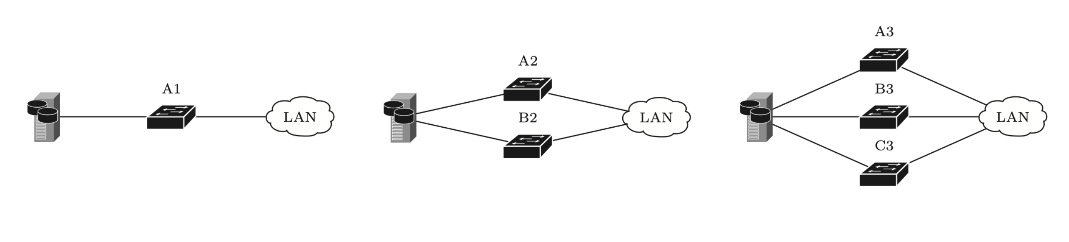
\includegraphics[scale=0.4]{study_case_model.png}
\end{center}
I dati del caso sono i seguenti:
\begin{itemize}
	\item Indici di \textbf{riciclabilità} $p_i$:
	\begin{itemize}
		\item \emph{Switch}: $0.7$
		\item \emph{Cavo}: $0.9$
	\end{itemize}
	dove durante il ciclo di vita un cavo e uno switch verranno sostituiti e alla fine i cavi saranno riusati e gli switch dismessi.
	\item \textbf{Potenza} assorbita da uno switch in un ciclo di vita di $3$ anni (con $\alpha = 0.389  \frac{kg CO_2-eq}{kWh}$):
	\begin{itemize}
		\item \emph{Costruzione} di uno switch $750kWh$ mentre di un cavo $1kWh$
		\item \emph{Smaltimento} di uno switch $400kWh$ mentre di un cavo $1kWh$
		\item \emph{Utilizzo} di uno switch $0.05kW$ da sommare a:
		\begin{itemize}
			\item $0.015kW$ per ogni porta usata al $100\%$ (porte 100 BaseT con uso medio di 10Mbps)
			\item $0.006kW$ per ogni porta idle 
		\end{itemize}
	\end{itemize}
	\item Probabilità di \textbf{fallimento} di uno switch o cavo ogni ora $10^{-5}$
	\item La \textbf{ridondanza} viene utilizzata solo quando necessario ed assumiamo quindi che sia sempre in idle
\end{itemize}
Di seguito lo svolgimento dei vari casi:
\begin{itemize}
	\item \textbf{Riciclabilità}
	\begin{equation*}
		\begin{split}
			& R_1 = \frac{0.7 + 0.7 +0.9}{3} = 0.767 = 76.7\%\\
			& R_2 = \frac{0.7+0.9 + 0.7 + 0.7}{4} = 0.75 = 75\% \\
			& R_3 = \frac{0.7 + 0.9 + 0.7 + 0.7 + 0.7}{5} = 0.74 = 74\%
		\end{split}
	\end{equation*}
	\newpage
	\item \textbf{Emissioni}
	\begin{itemize}
		\item Caso 1:
		\begin{equation*}
			\begin{split}
				& C_{switch_m} = 750kWh \cdot 2 \cdot \frac{0.389 \frac{kg CO_2-eq}{kWh}}{0.95} = 614.211 kg CO_w-eq\\
				& C_{switch_r} = 400 kWh \cdot 2 \cdot \frac{0.389 \frac{kg CO_2-eq}{kWh}}{0.95} = 327.579 kg CO_2-eq \\
				& C_{cavi_m} = 1kWh \cdot 3 \cdot \frac{0.389 \frac{kg CO_2-eq}{kWh}}{0.95}  = 1.228 kg CO_2-eq\\
				& C_{cavi_r} = 1kWh \cdot \frac{0.389 \frac{kg CO_2-eq}{kWh}}{0.95} = 0.409 kg CO_2-eq \\
				& C_{switch_u} = 0.015kW \cdot 2 \cdot \frac{0.389 \frac{kg CO_2-eq}{kWh}}{0.95} \cdot 8760\frac{h}{y} \cdot3y +\\
				 & + 0.05kW \cdot \frac{0.389 \frac{kg CO_2-eq}{kWh}}{0.95} \cdot 8760\frac{h}{y} \cdot 3 y= 860.877 kg CO_2-eq \\
				& C_{tot} = (614.211 + 327.579 + 1.228 + 0.409 + 860.877)kg CO_2-eq = \\
				& = 1804.304 kg CO_2-eq
			\end{split}
		\end{equation*}
		\item Caso 2:
		\begin{equation*}
			\begin{split}
				& C_{switch_m} = 750kWh \cdot 3 \cdot \frac{0.389 \frac{kg CO_2-eq}{kWh}}{0.95} = 921.316 kg CO_w-eq\\
				& C_{switch_r} = 400 kWh \cdot 3 \cdot \frac{0.389 \frac{kg CO_2-eq}{kWh}}{0.95} = 491.368 kg CO_2-eq \\
				& C_{cavi_m} = 1kWh \cdot 5 \cdot \frac{0.389 \frac{kg CO_2-eq}{kWh}}{0.95}  = 2.047 kg CO_2-eq\\
				& C_{cavi_r} = 1kWh \cdot \frac{0.389 \frac{kg CO_2-eq}{kWh}}{0.95} = 0.409 kg CO_2-eq \\
				& C_{switch_u} = 0.015kW \cdot 2 \cdot \frac{0.389 \frac{kg CO_2-eq}{kWh}}{0.95} \cdot 8760\frac{h}{y}\cdot 3y +\\
				& + 0.006kW \cdot 2 \cdot \frac{0.389 \frac{kg CO_2-eq}{kWh}}{0.95} \cdot 8760\frac{h}{y} \cdot 3y+ \\
				& + 0.05kW \cdot 2 \cdot \frac{0.389 \frac{kg CO_2-eq}{kWh}}{0.95} \cdot 8760\frac{h}{y} \cdot 3y= 1528.058 kg CO_2-eq \\
				& C_{tot} = (921.316 + 491.368 + 2.047 + 0.409 + 1528.058)kg CO_2-eq = \\
				& = 2943.198 kg CO_2-eq
			\end{split}
		\end{equation*}
		\item Caso 3:
		\begin{equation*}
			\begin{split}
				& C_{switch_m} = 750kWh \cdot 4 \cdot \frac{0.389 \frac{kg CO_2-eq}{kWh}}{0.95} = 1228.421 kg CO_w-eq\\
				& C_{switch_r} = 400 kWh \cdot 4 \cdot \frac{0.389 \frac{kg CO_2-eq}{kWh}}{0.95} = 655.158 kg CO_2-eq \\
				& C_{cavi_m} = 1kWh \cdot 7 \cdot \frac{0.389 \frac{kg CO_2-eq}{kWh}}{0.95}  = 2.866 kg CO_2-eq\\
				& C_{cavi_r} = 1kWh \cdot \frac{0.389 \frac{kg CO_2-eq}{kWh}}{0.95} = 0.409 kg CO_2-eq \\
				& C_{switch_u} = 0.015kW \cdot 2 \cdot \frac{0.389 \frac{kg CO_2-eq}{kWh}}{0.95} \cdot 8760\frac{h}{y} \cdot 3y+\\
				&+ 0.006kW \cdot 4 \cdot \frac{0.389 \frac{kg CO_2-eq}{kWh}}{0.95} \cdot 8760\frac{h}{y} \cdot 3y+ \\
				& + 0.05kW \cdot 3 \cdot \frac{0.389 \frac{kg CO_2-eq}{kWh}}{0.95} \cdot 8760\frac{h}{y} \cdot 3y= 2195.238 kg CO_2-eq \\
				& C_{tot} = (1228.421 + 655.158 + 2.866 + 0.409 + 2195.238)kg CO_2-eq =\\
				& = 4082.092 kg CO_2-eq
			\end{split}
		\end{equation*}
	\end{itemize}
	\item \textbf{Performance}: la probabilità che il sistema funzioni è
	\begin{equation*}
		(1-10^{-5})^3 = 0.99997
	\end{equation*}
	e quindi:
	\begin{equation*}
		\begin{split}
			& P_1 = (1-0.99997)^1 = 3 \cdot 10^{-5}\\
			& P_2 = (1-0.99997)^2 = 9 \cdot 10^{-10} \\
			& P_3 =(1-0.99997)^3 = 2.7 \cdot 10^{-14}
		\end{split}
	\end{equation*}
\end{itemize}
Concludendo, tutte le configurazioni rispettano il punto sulla \emph{riciclabilità}, nessuna quello sulle \emph{emissioni} e solo le ultime due quello sull'\emph{affidabilità}.
\end{document}
